\documentclass{article}
\usepackage[utf8]{inputenc}
\usepackage{hyperref}
\usepackage{bytefield}
\usepackage[
    type={CC},
    modifier={by-sa},
    version={4.0},
]{doclicense}

\title{
    \huge \textbf{BPX Format} \\
    \large \url{https://github.com/BlockProject3D/}
}
\author{Yuri Edward}
\date{04-28-2020}

\usepackage{natbib}
\usepackage{graphicx}
\usepackage[table]{xcolor}
\usepackage[margin=1in]{geometry}
\usepackage{amsmath}
\usepackage{titlesec}
\usepackage{fancyhdr}
\usepackage{tabulary}

\setlength{\arrayrulewidth}{0.5mm}
\setlength{\tabcolsep}{18pt}
\renewcommand{\arraystretch}{1.5}

% Heading
\pagestyle{fancy}
\fancyhf{}
\lhead{BlockProject Extended}
\rhead{Copyright (c) 2020, BlockProject 3D}
\rfoot{\thepage}
\lfoot{04-28-2020}

\begin{document}

\maketitle

\begin{figure}[h!]
    \centering
    
\includegraphics[scale=1.1]{logo}
    \label{fig:logo}
\end{figure}

\newpage

\begin{abstract}
    This document describes the BPX format, providing an optimized, flexible and DRM \cite{DRM} free storage designed for various multimedia content types commonly used in 3D applications.
\end{abstract}
\doclicenseThis

\section{Introduction}
When developing a 3D game engine there is often the problem of dealing with game modifications (mods). For example one might consider how easy it would be for the end player to add custom assets and/or change existing assets; whether the end player would need to agree against certain complex licenses or if it is even legally allowed to modify the content of certain asset files.\newline
Here the term asset refers to various types of files loaded by the game for a specific game world or for the entire game. These resources can be multimedia files, scripts, configurations and other formats the game engine could use.\newline
This format provides an alternative to existing asset formats geared towards the development of highly moddable, i.e. modify the game, add new assets, remove existing assets and/or change existing assets, and cross platform 3D games.\newline
The benefits are:
\begin{itemize}
    \item Open source with a permissive licence.\newline
    Redistribute source code, allow improvements of the format by others.
    \item DRM \cite{DRM} free.\newline
    Avoid licensing problems and restrictions. DRM stands for Digital Rights Management and is used to control how the user is allowed to interact with certain multimedia content. In moddable games DRM usually restricts the user from modifying existing assets.
    \item Flexible.\newline
    Designed for providing support for moddability. The nature of container allows support of all kinds of multimedia resources used in a typical real-time 3D application.
    \item Optimized for 3D APIs such as OpenGL \cite{OpenGL}, DirectX \cite{DirectX}, Vulkan \cite{Vulkan}\newline
    Certain types of BPX use some assumptions on the input data in order to reduce pre-process time when loading assets in a typical real time rendering engine.
    \item Cross platform.\newline
    Can store data for compatibility over multiple platforms within a single file due to its nature of containers.
\end{itemize}

\section{History}
The BPX format also refered to BlockProject Extended is a remake of an old format designed for the first version of the BlockProject 3D engine as an attempt to allow moddability, that means change the behaviour of a game while it's running and in this case change also any multimedia asset including scenes, shaders, models and even textures...\newline
This has proved to be a difficult task due to licensing issues, restrictions imposed by existing frameworks and restrictions imposed by certain formats.\newline
As a result a custom asset format has been developed for initially a very limited set of type of assets in order to solve the issue.\newline
This format is an evolution geared towards re-usability and performance.

\section{Comparison against mainstream formats}
Below is a non-exhaustive table showing the differences between the idea of BPX and existing mainstream formats:
\bpxtable{C|c|c|c|c|c}{Name & Open & DRM & Flexible & Optimized & Compat.}
{
    FBX & \cellcolor{red}No & \cellcolor{green}No & \cellcolor{red}No & \cellcolor{green}Yes & \cellcolor{yellow}Partial \\
    Unreal & \cellcolor{red}No & \cellcolor{red}Yes & \cellcolor{green}Yes & \cellcolor{green}Yes & \cellcolor{yellow}Partial \\
    Unity & \cellcolor{red}No & \cellcolor{red}Yes & \cellcolor{yellow}Partial & \cellcolor{green}Yes & \cellcolor{yellow}Partial \\
    OBJ & \cellcolor{green}Yes & \cellcolor{green}No & \cellcolor{red}No & \cellcolor{red}No & \cellcolor{green}Yes \\
}
\begin{itemize}
    \item FBX: It is possible to save files as Text based FBX however no open documentation exists for the format. The binary FBX requires the use of a closed source library. FBX supports Windows without issues, however getting the SDK to work on different platforms might be an issue.\newline
    FBX is designed to support 3D models.
    \item The source code of Unreal can be accessed if you agree to certain licenses which prohibit the redistribution of the editor source code in the game, preventing the use of Unreal's format as a base to support modding. Also Unreal does not provide easy installation under Linux.\newline
    Unreal is also using a unified format for all assets of the game. It has support for modding however the modder is required to agree to licenses and to download the full SDK.
    \item Unity, although it has better support for Linux, might still be a bit tricky in certain combinations of distribution/system.\newline
    Unity is also using a unified format for all assets of the game but the game engine does not allow load of arbitrary custom assets. The asset format used by unity is also closed and does not permit modification by the player of the game like Unreal.
    \item OBJ is a text based 3D model format. The format has no support for skeletal based models/animations and has poor support for materials.
\end{itemize}
\section{General}
The format is based on the idea of a container with a reusable main header that can be extended for the different applications. While each BPX type defines it's own set of sections to load to comply to that given type, an implementation must be able to support any number of additional custom sections, even if those are not used in the application.\newline
The following assumptions are used:
\begin{itemize}
    \item A byte is assumed to be 8 bits.
    \item The sizes are expressed in bits in the entire document.
    \item The byte order in a BPX file should be \textbf{little endian} to match most of current hardware/software architectures, and then avoid a pre-processing step when loading the file.
    \item A transformation is stored in terms of float to match most current rendering APIs.
    \item The coordinate system used for this format is assumed to be right handed with the Z axis to be pointing upward.
\end{itemize}
Description of the coordinate system:
\begin{equation}
    Right =
    \begin{pmatrix}
        1 \\
        0 \\
        0
    \end{pmatrix}
    Forward =
    \begin{pmatrix}
        0 \\
        1 \\
        0
    \end{pmatrix}
    Up =
    \begin{pmatrix}
        0 \\
        0 \\
        1
    \end{pmatrix}
\end{equation}
The TypeExt section available in certain BPX types describes what fields to expect in the 128 bits of extension located in the BPX Main Header.\newline
If the TypeExt field isn't used by a specific BPX type then this field should be set to 0.

\section{Padding rules}
All data structures exposed in this format specification are padded to comply with major C/C++ compilers: Visual C++, GCC and Clang.

\section{Floating points}
All floating points in this format are stored in IEEE 754 format \cite{ieee754}.

\section{Hashing function}
Some types of BPX requires hashing for some strings. The string hash function to apply is defined by:

\begin{equation}
	h_X(0) = 5381
\end{equation}
\begin{equation}
	h_X(n + 1) = \left( \left( h_X(n) \times 2^5 \right) + h_X(n) \right) + X_{n + 1}
\end{equation}
where $X$ is a row vector containing the raw bytes of the string.
\section{BPX Main Header}
The BPX Main Header describes general information about the container and the contained data.\newline
This section is \textbf{not compressable}.\newline
Below is a table describing the different fields to be expected in the header:
\begin{center}
    {
        \rowcolors{2}
        {red!15}
        {blue!15}
        \begin{tabular}{|c|c|c|c|}
            \hline
            \textbf{Name} & \textbf{Type} & \textbf{Size} & \textbf{Notes} \\
    
            \hline\hline
            Signature & String & 24 & File signature; always "BPX" \\
            Type & Unsigned & 8 & Type of BPX \\
            Chksum & Unsigned & 32 & Checksum \\
            FileSize & Unsigned & 64 & Size of file after compression \\
            SectionNum & Unsigned & 32 & Number of sections \\
            Version & Unsigned & 32 & Version of format \\
            TypeExt & Unspecified & 64 & Extension space for various BPX types \\
            \hline
        \end{tabular}
    }
\end{center}
\begin{center}
    \begin{bytefield}[bitwidth=0.73em]{64}
        \bitheader{0-63} \\
        \bitbox{24}{Signature} & \bitbox{8}{Type} & \bitbox{32}{Chksum} \\
        \bitbox{64}{FileSize} \\
        \bitbox{32}{SectionNum} & \bitbox{32}{Version} \\
        \bitbox{64}{TypeExt}
    \end{bytefield}
\end{center}

\subsection{Signature}
Three characters to describe the file when open in a text/hex editor

\subsection{Type}
The type of BPX. This is used to describe what type of sections to expect in the file.\newline
Currently only the following are supported:
\begin{itemize}
    \item 'T' for Texture
    \item 'M' for Model
    \item 'S' for Shader
    \item 'C' for Scene
    \item 'P' for Package
\end{itemize}
Here the characters between single quotes are to interpreted as their byte representation in ASCII encoding.

\subsection{Version}
Version of the file, the currently only available version of the format is 0.

\subsection{SectionNum}
Number of sections in the file.

\subsection{Chksum}
Checksum calculated with the help of a CRC32 algorithm. This should integrate both the header (except for the Chksum field) and the file content after compression.

\subsection{FileSize}
The file size field corresponds to the total size of the file minus the size of the header in bytes after compression; this is used as an additional security over the integrity of the file. It can also be used to check the remaining number of bytes in a network based streaming application.

\subsection{TypeExt}
The TypeExt field provides 64 bits of extension for different kind of BPX avoiding having to store or load additional sections in order to get usefull general information about a specific file reducing load time and memory complexity.\newline
All unused space in this field should be 0.

\section{BPX Section Header Table}
The BPX Section Header Table is an array of data structures describing important information for each section present in the file. It is located after the BPX Main Header.\newline
The size of this array is determined by the SectionNum field in the BPX Main Header. The array is expected to be contiguous.\newline
Certain types of BPX expects to be able to index sections in this table using positions. For that reason, the array is expected to be 1-indexed to allow for a value of 0 to represent a null or non-existent section.\newline
This section is \textbf{not compressable}.

\subsection{BPX Section Header}
Below is a table describing the feilds to expect in a BPX Section Header:

\bpxfieldtable
{
    Pointer & Unsigned & 64 & Offset in bytes from the beginning of the file \\
    CSize & Unsigned & 32 & Size in bytes of section (compressed) \\
    USize & Unsigned & 32 & Size in bytes of section (uncompressed) \\
    Chksum & Unsigned & 32 & Checksum \\
    Type & Unsigned & 8 & Type of Section \\
    Flags & Unsigned & 8 & Flags for the current section \\
    Reserved & Unspecified & 16 & Blank, always 0 \\
}
\begin{center}
    \begin{bytefield}[bitwidth=0.73em]{64}
        \bitheader{0-63} \\
        \bitbox{64}{Pointer} \\
        \bitbox{32}{CSize} & \bitbox{32}{USize} \\
        \bitbox{32}{Chksum} & \bitbox{8}{Type} & \bitbox{8}{Flags} & \bitbox{16}{Reserved}
    \end{bytefield}
\end{center}

\subsubsection{Pointer}
Position in bytes in the file where the content for a given section should be found.

\subsubsection{CSize}
Size in bytes of the content after compression for a given section excluding Section Header.

\subsubsection{USize}
Size in bytes of the content before compression for a given section excluding Section Header.

\subsubsection{Chksum}
Checksum of uncompressed data, refer to the Check type of flags in the flags sub-section (\ref{sssec:Flags}) to know how to interpret and generate this field. If no checksum flag is specified, the checksum is ignored.

\subsubsection{Type}
An integer to represent the type of section.

\subsubsection{Flags} \label{sssec:Flags}
Bit mask based flags (or flags together). Currently the only supported flags are:
\bpxtable{c|c|C}{Name & Value & Notes}
{
    CompressedZlib & 0x1 & Indicates the section is compressed using the zlib \cite{zlib} algorithm \\
    CompressedXZ & 0x2 & Indicates the section is compressed using the XZ \cite{xz} algorithm \\
    CheckCrc32 & 0x4 & Indicates the section checksum is computed using Crc32 algorithm \\
    CheckWeak & 0x8 & Indicates the section checksum is computed with the weak variant as used in the BPX Main Header \\
}


\section{BPX Type: Texture ('T')}

\subsection{Overview}
The Texture BPX is using 'T' as the type byte of BPX Main Header. This type provides optimized and efficient texture storage for 3D rendering APIs.
\newline
Below is a table describing the different sections to be expected in a BPXT:
\begin{center}
    {
        \rowcolors{2}
        {red!15}
        {blue!15}
        \begin{tabular}{|c|c|c|c|}
            \hline
            \textbf{Name} & \textbf{Type} & \textbf{Required} & \textbf{Single Time} \\

            \hline\hline
            PixelArray & 0 & Yes & Yes \\
            \hline
        \end{tabular}
    }
\end{center}

\subsection{TypeExt}
Contains information about the texture encoding.
\begin{center}
    {
        \rowcolors{2}
        {red!15}
        {blue!15}
        \begin{tabular}{|c|c|c|c|}
            \hline
            \textbf{Name} & \textbf{Type} & \textbf{Size} & \textbf{Notes} \\
    
            \hline\hline
            Width & Unsigned & 4 & Texture width \\
            Height & Unsigned & 4 & Texture height \\
            Format & Unsigned & 4 & Texture format \\
            Flags & Unsigned & 4 & Flags \\
            MipMap Level & Unsigned & 8 & Number of mip maps \\
            Array & Unsigned & 16 & Size of texture array (0 = no texture array) \\
            \hline
        \end{tabular}
    }
\end{center}

\subsubsection{Width}
The expected width of all pixel arrays in power of two form ($2^{k+1}$px where k is the stored number).

\subsubsection{Height}
The expected height of all pixel arrays in power of two form ($2^{k+1}$px where k is the stored number).

\subsection{Analysis on texture size storage}
Certain redering APIs requires that the textures are aligned to a specific implementation defined number of pixels per row. This number also called stride is usualy 8 or a power of two greater than 8.\newline
By assuming any BPX encoded texture is encoded with power of twos instead of their actual resolution in pixels, we can eliminate the need, in the cases where the implementation uses power of two strides, to run a padding alignment before presenting the texture to this implementation. Also this allows to reduce the field size for storing texture size: instead of using 32 bits or 64 bits we can store a texture size in 8 bits and keep relatively large texture sizes, \textbf{optimizing both storage space and application load speed}. Indeed the maximum texture size in each direction allowed by BPX would be $2^{15 + 1} = 2^{16} = 65536$. Most rendering API implementation do not support such large texture sizes.\newline
From there one might say that we should then use less than 8 bits. However using less than 8 bits for storing the entire size vector would conflict with hardware indexing as most hardware only indexes 8 bits bytes.

\subsubsection{Format}
Available formats:
\begin{center}
    {
        \rowcolors{2}
        {red!15}
        {blue!15}
        \begin{tabular}{|c|c|c|c|}
            \hline
            \textbf{Name} & \textbf{Value} & \textbf{Notes} \\

            \hline\hline
            RGB & 0x1 & Standard 8 bits 3 channel RGB format \\
            RGBA & 0x2 & 8 bits 4 channel RGB with transparency level \\
            GREY\_SCALE & 0x3 & Single 8 bits channel representing grey scale level \\
            FLOAT & 0x4 & Single channel 32 bits float texture \\
            \hline
        \end{tabular}
    }
\end{center}

\subsubsection{Flags}
Bit mask based flags (or flags together). Currently the only supported flags are:
\begin{center}
    {
        \rowcolors{2}
        {red!15}
        {blue!15}
        \begin{tabular}{|c|c|c|}
            \hline
            \textbf{Name} & \textbf{Value} & \textbf{Notes} \\
    
            \hline\hline
            Array & 0x1 & Indicates the texture should be interpreted as a texture array \\
            Compressed & 0x2 & Indicates the texture should be GPU compressed on load \\
            CubeMap & 0x4 & Indicates the texture should be interpreted as a CubeMap \\
            \hline
        \end{tabular}
    }
\end{center}

\subsubsection{MipMap Level}
Number of mip maps \cite{MipMap} to auto generate when loading this texture.

\subsubsection{Array}
Number of textures for creating a texture array. If this value is 0 consider this is not a texture array.\newline
Ignore this value if neither of Array or CubeMap flags are set.

\subsection{PixelArray}
Texture data array encoded as described by texture format.\newline
If the \textit{Array} value in the header is greater than 0 then a series of \textit{Array} count texture data arrays are saved one after the other encoded with respect to the texture format described by the header.\newline
In case the CubeMap flag is set the \textit{Array} field in the header should be 6 and this section should contain 6 texture data arrays.
\section{BPX Type: Model ('M')}

\subsection{Overview}
The Model BPX is using 'M' as the type byte of BPX Main Header. This type provides optimized and efficient mesh storage for 3D rendering APIs.
\newline
Below is a table describing the different sections to be expected in a BPXM:
\bpxsectiontable
{
    VertexArray & 2 & Yes & No \\
    IndexArray & 3 & No & No \\
    BoneArray & 4 & No & Yes \\
    FrameArray & 5 & No & Yes \\
    AnimationArray & 6 & No & Yes \\
    Strings & 255 & No & Yes \\
}

\subsection{TypeExt}
Contains general information about the 3D model file.
\bpxfieldtable
{
    VertexFormatHash64 & Unsigned & 64 & Hash of vertex format \\
    VertexFormatHash32 & Unsigned & 32 & Hash of vertex format \\
    Reserved & Unspecified & 32 & Blank, always 0 \\
}
\begin{center}
    \begin{bytefield}[bitwidth=1.2em]{32}
        \bitheader{0-31} \\
        \begin{rightwordgroup}{128 bits}
            \bitbox{32}{VertexFormatHash64} \\
            \bitbox{32}{VertexFormatHash64} \\
            \bitbox{32}{VertexFormatHash32} \\
            \bitbox{32}{Reserved}
        \end{rightwordgroup}
    \end{bytefield}
\end{center}

\subsubsection{VertexFormatHash64}
64 bits hash of vertex format asset virtual path corresponding to the vertex structure that this shader expects as input.

\subsubsection{VertexFormatHash32}
32 bits hash of vertex format asset virtual path corresponding to the vertex structure that this shader expects as input.

\subsubsection{VertexFormat}
The actual definition of the vertex format is specified as a separate asset, left to the implementation for flexibility.

\subsection{VertexArray}
This section contains a header followed by an array of vertex data structure. The size of each vertex structure should be equal to the field VertexSize in the VertexFormat section.\newline
The header data structure is described in the following table:
\bpxfieldtable
{
    MaterialHash64 & Unsigned & 64 & Hash of material \\
    MaterialHash32 & Unsigned & 32 & Hash of material \\
    VertexCount & Unsigned & 32 & Total number of vertices \\
    IndexArray & Unsigned & 32 & Index array section index \\
}
\begin{center}
    \begin{bytefield}[bitwidth=1.1em]{32}
        \bitheader{0-31} \\
        \bitbox{32}{Material} \\
        \bitbox{32}{VertexCount} \\
        \bitbox{32}{IndexArray}
    \end{bytefield}
\end{center}

\subsubsection{MaterialHash64}
64 bits hash of material asset virtual path to apply by default to this vertex array.

\subsubsection{MaterialHash32}
32 bits hash of material asset virtual path to apply by default to this vertex array.

\subsubsection{VertexCount}
The amount of vertex structures to read after this header.\newline
\textbf{We remind that all modern hardware support triangles as primitives, so the vertex count should be a multiple of 3}

\subsubsection{IndexArray}
This field is an index in the section header table to an IndexArray that should be used alongside this VertexArray.\newline
A value of $0$ means that no IndexArray is associated to that VertexArray.

\subsubsection{Total array size}
The total size in bytes of the vertex array to use as pre-allocation buffer size when loading this model can be calculated as follows:
\begin{equation}
    SA = S \times V
\end{equation}
where $SA$ is the total size of the vertex array, $S$ the size of a single vertex structure as given in the VertexFormat asset and $V$ the number of vertices in the array given by the VertexCount field.\newline
To avoid storing an additional 64 bits field in the header of the VertexArray section this size $SA$ is left to be calculated by the implementing application.

\subsection{IndexArray}
The index array section allows to ommit certain vertices and figure out these vertices at runtime. Instead of writing all vertices for a given model requiring more space to store them, we only store unique vertices, and duplicates are just resolved by matching a vertex index from this section to an actual vertex structure, \textbf{this allows to save storage space and RAM}.\newline
This section contains a header describing the amount of indices to be found in the array, and an array of 32 bits unsigned integer each representing the index of a vertex in a given vertex array.\newline
Below is a table describing the data structure to expect as header for an IndexArray section:
\bpxfieldtable
{
    IndexCount & Unsigned & 32 & Total number of indices \\
}

\subsubsection{IndexCount}
The number of indices expected to be read from the array below this header.

\subsection{BoneArray}
This section contains a header followed by an array of data structures representing each bone in a skeletal mesh.\newline
Below is a description of the header to find before bone data in this section:
\bpxfieldtable
{
    BoneCount & Unsigned & 16 & Total number of bones \\
}

Each bone in the array following the header is represented by the following data structure:
\bpxfieldtable
{
    Head & 3D float vector & 96 & Initial position of bone head \\
    Tail & 3D float vector & 96 & Initial position of bone tail \\
    Name & Unsigned & 32 & Pointer in the Strings section \\
}
\begin{center}
    \begin{bytefield}[bitwidth=1.1em]{32}
        \bitheader{0-31} \\
        \bitbox{32}{Head [3]} \\
        \bitbox{32}{Tail [3]} \\
        \bitbox{32}{Name}
    \end{bytefield}
\end{center}

\subsubsection{BoneCount}
Number of bones to expect in the bone array following the header. This number should belong to the interval $[1, 1024]$.

\subsection{Analysis on theoretical bone limit}
We can give an estimation that human skeleton can be up to 400 bones. Of course most models do not include as many bones to reduce GPU/CPU load.
\begin{itemize}
    \item OpenGL, Vulkan and Metal maximum UBO/function constants storage size available to a shader is usualy 64Kb or 65536 bytes
    \item On the official MSDN page \cite{MSDNConstantBuffers} for DirectX the maximum constant buffer size available to a shader is $4096 constants \times 4 \times 32 bits = 4096 constants \times 16 bytes = 65536 bytes$
\end{itemize}
UBO, function constants and constant buffer refers to means of variable synchronisation between CPU accessible memory and GPU accessible memory. Vulkan is a special case as it actually supports faster memory called Push Constants, however these constants usually maxes at 256-512 bytes which is impracticable for storing bone transforms. Push constants are typically used to exchange important transformation matrices such as model, view or projection.
The size of a transformation matrix in 3D space using homogeneous coordinate system \cite{HomogeneousCoordinates} is $32 bits (float) \times 4 \times 4 (4\times4 matrix) = 16 \times 32 bits = 512 bits = 64 bytes$.\newline
So assuming the lowest size for storing bones in VRAM for GPU processing is $65536$ we can theoretically store up to $1024$ matrices assuming each bone matrix represents 3D space transformations in homogeneous coordinate system ($\frac{65536}{64} = 1024$).\newline
Which means in order to \textbf{keep compatibility} with as many platforms/rendering apis as possible also taking into account byte indexing, we should store the bone count as a 16 bits integer.

\subsubsection{Head}
Initial head position for that specific bone.

\subsubsection{Tail}
Initial tail position for that specific bone.

\subsubsection{Name}
Bone name as a pointer to a null terminated string in the strings section.

\subsection{FrameArray}
This section contains a header followed by an array of data structures each representing the new transform for a combination of a bone and frame.\newline
The array should be organized as the following diagram describes:
\begin{figure}[h!]
    \centering
    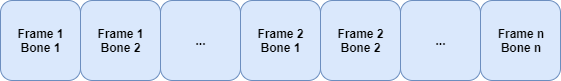
\includegraphics[scale=0.7]{Types/FrameArray_Diagram.png}
    \label{fig:FrameArray_Diagram}
    \caption{Diagram for organizing frame array}
\end{figure}
\newline
A single animation in a 3D model is usualy a set of actions. For example consider the following set of actions on a 3D human based model:
\begin{itemize}
    \item move left leg
    \item move right leg
    \item move left arm
    \item move right arm
\end{itemize}
This set of actions could be grouped together in one animation named walking or running.\newline
We call total animation time, the total time needed to express all animations for a single 3D model.

\subsubsection{Design decision}
The majority of mainstream formats represents animated models using key frames, that is storing only determinant changes in the model and interpolating intermediate frames at runtime (either when loading the file or while rendering). In BPX type M each frame is stored in the file to allow for any interpolation method, that is the interpolation if there's any is defined by the exporter of that model. The engine runtime does not have to provide any interpolation function for BPX type M.\newline
This change grants the \textbf{flexibility} of using any interpolation functions even user defined.

\subsubsection{Analysis on theoretical required storage size}
We assume the total size required to store the full FrameArray is given by the following formula:
\begin{equation}
    F \times B \times B_s
\end{equation}
where $F$ is the total amount of frames, $B$ the number of bone updates per frame and $B_s$ is the size of a single bone update structure.\newline
We previously indicated that a bone update is determined by a transformation matrix in homogeneous coordinate space \cite{HomogeneousCoordinates}, that means it is exactly $512bits$ or $64bytes$.\newline
Of course in a real application, it is very unlikely to have every frame in the timeline requiring update on every bone.
\vspace{12pt}
\newline\textbf{Worst case scenario}\newline
We assume the total animation time won't exceed $4$ minutes.\newline
We showed earlier that the theoretical maximum bone limit is $1024$.\newline
For the frame rate we choose $60$, that means each second $60$ frames in this FrameArray have to be rendered.\newline
The total amount of frames to store is $60 \times 4 \times 60 = 14400frames$.\newline
The total size required to save a model assuming each frame requires dependency over exactly all bones is $14400 \times 1024 \times 512 = 7549747200bits = 943718400bytes$. That is approximately $944Mb$.
\vspace{12pt}
\newline\textbf{Average case scenario}\newline
Of course having $1024$ bones in one model is unlikely to happen. This is why we want to have an average estimation on the size required to store the FrameArray section.\newline
On average, the amount of bones per animated model won't exceed $50$ bones.\newline
On average, each frame will update at most $10$ bones.\newline
On average, the frame rate of a 3D model animation will be $30FPS$.\newline
On average, the total animation time won't exceed $2$ minutes.\newline
The total amount of frames to store is $30 \times 2 \times 60 = 3600frames$.\newline
The total size required to save the FrameArray of a model assuming each frame requires dependency over exactly all bones is $3600 \times 10 \times 512 = 18432000bits = 2304000bytes$. That is approximately $2Mb$.
\vspace{12pt}
\newline
In conclusion the FrameArray section \textbf{should be compressed} to reduce the storage space consumed by a single model asset on disk. When loading the model in RAM one might consider adding some compression or supporting a lower limit than $1024$ bones.

\subsubsection{Bone transform}
Each bone transformation in the FrameArray section is represented by the following structure:
\bpxfieldtable
{
    Rotation & 4D float vector & 128 & Target bone rotation as a quaternion \\
    Position & 3D float vector & 96 & Target bone position \\
    Scale & 3D float vector & 96 & Target bone scale \\
    BoneId & Unsigned & 32 & Index of affected bone \\
}
\begin{center}
    \begin{bytefield}[bitwidth=1.1em]{32}
        \bitheader{0-31} \\
        \bitbox{32}{Rotation [4]} \\
        \bitbox{32}{Position [3]} \\
        \bitbox{32}{Scale [3]} \\
        \bitbox{32}{BoneId}
    \end{bytefield}
\end{center}

\subsection{Strings}
The strings section contains a list of null-terminated strings to be referenced by start offset from other sections.
\section{BPX Type: Shader Package ('S')}

\subsection{Overview}
The Shader Package BPX is using 'S' as the type byte of BPX Main Header. This type provides optimized and cross API/platform storage for rendering code intended to be executed on the GPU \cite{GPU}.
\newline
Below is a table describing the different sections to be expected in a BPXS:
\begin{center}
    {
        \rowcolors{2}
        {red!15}
        {blue!15}
        \begin{tabular}{|c|c|c|c|}
            \hline
            \textbf{Name} & \textbf{Type} & \textbf{Required} & \textbf{Single Time} \\
    
            \hline\hline
            Shader & 1 & Yes & No \\
            Assembly & 2 & Yes & No \\
            Bindings & 3 & Yes & No \\
            MaterialConstants & 4 & Yes & Yes \\
            Strings & 255 & Yes & Yes \\
            \hline
        \end{tabular}
    }
\end{center}
At least one assembly section is required to be saved in the file.

\subsubsection{Design decisions}
The shader type has been designed to store different versions of a single shader but conpiled against different rendering APIs.\newline
For this reason, each rendering API should load the shaders composing the program by referring to it's Assembly section.\newline
The assembly section also contains required information when loading a shader program.\newline
In order to account for cases where it is not possible to provide version for each rendering API of a given shader, the shader program BPX contains a bit mask field to indicate compatibility or incompatibility against a given rendering API.\newline
For example a shader compiled under Linux won't have DirectX shader byte code, it can store the source code HLSL (High Level Shading Language is Microsoft's shading language for DirectX) however not all DirectX enabled systems can compile shaders on the fly.\newline
In conclusion, for \textbf{better compatibility} it is recommended to build shaders under Windows, for the \textbf{best compatibility} a Mac will be needed in order to build shaders for MSL (Metal Shading Language is Apple's shading language for Metal API).

\subsection{TypeExt}
Contains information about the shader package.
\begin{center}
    {
        \rowcolors{2}
        {red!15}
        {blue!15}
        \begin{tabular}{|c|c|c|c|}
            \hline
            \textbf{Name} & \textbf{Type} & \textbf{Size} & \textbf{Notes} \\
    
            \hline\hline
            VertexFormatHash64 & Unsigned & 64 & Hash of vertex format \\
            VertexFormatHash32 & Unsigned & 32 & Hash of vertex format \\
            CompatibilityFlags & Unsigned & 8 & Flags \\
            NumConstants & Unsigned & 8 & Number of constants \\
            Reserved & Unspecified & 16 & Blank, always 0 \\
            \hline
        \end{tabular}
    }
\end{center}
\begin{center}
    \begin{bytefield}[bitwidth=1.2em]{32}
        \bitheader{0-31} \\
        \begin{rightwordgroup}{128 bits}
            \bitbox{32}{VertexFormatHash64} \\
            \bitbox{32}{VertexFormatHash64} \\
            \bitbox{32}{VertexFormatHash32} \\
            \bitbox{8}{CompatibilityFlags} & \bitbox{8}{NumConstants} & \bitbox{16}{Reserved}
        \end{rightwordgroup}
    \end{bytefield}
\end{center}

\subsubsection{VertexFormatHash64}
64 bits hash of vertex format asset virtual path corresponding to the vertex structure that this shader expects as input.

\subsubsection{VertexFormatHash32}
32 bits hash of vertex format asset virtual path corresponding to the vertex structure that this shader expects as input.

\subsubsection{CompatibilityFlags}
Bit mask based flags (or flags together). These flags are used to check if a given shader program can be used with the current configuration of hardware/driver/rendering implementation. By default packages compiled from BPSL will be compatible with OpenGL 3.0 and greater; DirectX 11 and 12 will be supported if the compiling machine has Windows and the DirectX SDK (the DirectX SDK is not available on Linux/Mac/etc).\newline
Currently the only supported flags are:
\begin{center}
    {
        \rowcolors{2}
        {red!15}
        {blue!15}
        \begin{tabular}{|c|c|c|}
            \hline
            \textbf{Name} & \textbf{Value} & \textbf{Notes} \\
    
            \hline\hline
            DirectX & 0x1 & Indicates compatibility with DirectX \cite{DirectX} \\
            OpenGL & 0x2 & Indicates compatibility with OpenGL \cite{OpenGL} \\
            Vulkan & 0x4 & Indicates compatibility with Vulkan \cite{Vulkan} \\
            Metal & 0x8 & Indicates compatibility with Metal \cite{Metal} \\
            \hline
        \end{tabular}
    }
\end{center}

\subsubsection{NumConstants}
Number of constant description structures in the MaterialConstants section.

\subsection{Shader}
Contains shader data for a single rendering API...\newline
A shader package can contain multiple shaders.

\subsection{Assembly}
Contains the shader list, order and other linking information for use by a rendering API.
Below is a table describing the data structure to expect in this section:
\begin{center}
    {
        \rowcolors{2}
        {red!15}
        {blue!15}
        \begin{tabular}{|c|c|c|c|}
            \hline
            \textbf{Name} & \textbf{Type} & \textbf{Size} & \textbf{Notes} \\

            \hline\hline
            Driver & Unsigned & 8 & Target driver of this assenbly \\
            Reserved & Unspecified & 24 & Blank, always 0 \\
            MinVersion & Unsigned & 32 & Minimum supported version \\
            VertexShaderId & Unsigned & 32 & Vertex shader section index \\
            DomainShaderId & Unsigned & 32 & Domain shader section index \\
            HullShaderId & Unsigned & 32 & Hull shader section index \\
            GeometryShaderId & Unsigned & 32 & Geometry shader section index \\
            PixelShaderId & Unsigned & 32 & Pixel shader section index \\
            Bindings & Unsigned & 32 & Number of bindings \\
            BindingsId & Unsigned & 32 & Bindings section id \\
            \hline
        \end{tabular}
    }
\end{center}
\begin{center}
    \begin{bytefield}[bitwidth=1.4em]{32}
        \bitheader{0-31} \\
        \bitbox{8}{Driver} & \bitbox{24}{Reserved} \\
        \bitbox{32}{MinVersion} \\
        \bitbox{32}{VertexShaderId} \\
        \bitbox{32}{HullShaderId} \\
        \bitbox{32}{DomainShaderId} \\
        \bitbox{32}{GeometryShaderId} \\
        \bitbox{32}{PixelShaderId} \\
        \bitbox{32}{Bindings} \\
        \bitbox{32}{BindingsId}
    \end{bytefield}
\end{center}
All indexes are given as positions in the Section Header Table.

\subsubsection{Driver}
The target rendering API for this assembly. List of possible values:
\begin{center}
    {
        \rowcolors{2}
        {red!15}
        {blue!15}
        \begin{tabular}{|c|c|c|c|}
            \hline
            \textbf{Name} & \textbf{Value} \\

            \hline\hline
            OpenGL & 0 \\
            DirectX & 1 \\
            Vulkan & 2 \\
            Metal & 3 \\
            \hline
        \end{tabular}
    }
\end{center}

\subsubsection{MinVersion}
The minimum supported version for this shader. This value is dependent over the target rendering API supported by the assembly. Refer to the rendering API implementation for information on how the minimum version is encoded.

\subsection{Bindings}
The bindings section stores information about what bindings are used in this shader assembly for a particular rendering API.\newline
This section stores an array of binding structures. A binding structure is defined by:
\begin{center}
    {
        \rowcolors{2}
        {red!15}
        {blue!15}
        \begin{tabular}{|c|c|c|c|}
            \hline
            \textbf{Name} & \textbf{Type} & \textbf{Size} & \textbf{Notes} \\

            \hline\hline
            StageFlags & Signed & 32 & Stage flags \\
            Type & Unsigned & 8 & Type of binding \\
            Register & Unsigned & 8 & Register number \\
            Reserved & Unspecified & 16 & Blank, always 0 \\
            \hline
        \end{tabular}
    }
\end{center}
\begin{center}
    \begin{bytefield}[bitwidth=1.4em]{32}
        \bitheader{0-31} \\
        \bitbox{32}{StageFlags} \\
        \bitbox{8}{Type} & \bitbox{8}{Register} & \bitbox{16}{Reserved}
    \end{bytefield}
\end{center}

\subsubsection{StageFlags}
Describes to what stage this binding is acceptable. These flags are bit mask that can be or'ed together in order to map to multiple stages. Below is a table to list the different available flags:
\begin{center}
    {
        \rowcolors{2}
        {red!15}
        {blue!15}
        \begin{tabular}{|c|c|c|}
            \hline
            \textbf{Name} & \textbf{Value} & \textbf{Notes} \\
    
            \hline\hline
            LOCK\_VERTEX\_STAGE & 0x1 & Indicates binding locks to vertex shader \\
            LOCK\_HULL\_STAGE & 0x2 & Indicates binding locks to hull shader \\
            LOCK\_DOMAIN\_STAGE & 0x4 & Indicates binding locks to domain shader \\
            LOCK\_GEOMETRY\_STAGE & 0x8 & Indicates binding locks to geometry shader \\
            LOCK\_PIXEL\_STAGE & 0x10 & Indicates binding locks to pixel shader \\
            \hline
        \end{tabular}
    }
\end{center}

\subsubsection{Type}
The type of binding. Currently there are only 4 types of binding:
\begin{center}
    {
        \rowcolors{2}
        {red!15}
        {blue!15}
        \begin{tabular}{|c|c|c|c|}
            \hline
            \textbf{Name} & \textbf{Value} \\

            \hline\hline
            TEXTURE & 0 \\
            SAMPLER & 1 \\
            CONSTANT\_BUFFER & 2 \\
            FIXED\_CONSTANT\_BUFFER & 3 \\
            \hline
        \end{tabular}
    }
\end{center}

\subsection{MaterialConstants}
The Material structure expected by this shader. Like for the binding section, this section is also a contiguous array of constant description structures. A constant description structure is defined as follows:
\begin{center}
    {
        \rowcolors{2}
        {red!15}
        {blue!15}
        \begin{tabular}{|c|c|c|c|}
            \hline
            \textbf{Name} & \textbf{Type} & \textbf{Size} & \textbf{Notes} \\

            \hline\hline
            Name & Unsigned & 32 & Name of constant \\
            Type & Unsigned & 8 & Type of constant \\
            Reserved & Unspecified & 24 & Blank, always 0 \\
            \hline
        \end{tabular}
    }
\end{center}
\begin{center}
    \begin{bytefield}[bitwidth=1.4em]{32}
        \bitheader{0-31} \\
        \bitbox{32}{Name} \\
        \bitbox{8}{Type} & \bitbox{24}{Reserved}
    \end{bytefield}
\end{center}

\subsubsection{Name}
The name of the constant as an offset pointer in the string section.

\subsection{Type}
The type of constant. Below is an exhaustive table of all accepted types:
\begin{center}
    {
        \rowcolors{2}
        {red!15}
        {blue!15}
        \begin{tabular}{|c|c|c|c|}
            \hline
            \textbf{Name} & \textbf{Value} \\

            \hline\hline
            FLOAT & 0 \\
            VECTOR\_FLOAT\_2 & 1 \\
            VECTOR\_FLOAT\_3 & 2 \\
            VECTOR\_FLOAT\_4 & 3 \\
            INT & 4 \\
            VECTOR\_INT\_2 & 5 \\
            VECTOR\_INT\_3 & 6 \\
            VECTOR\_INT\_4 & 7 \\
            UINT & 8 \\
            VECTOR\_UINT\_2 & 9 \\
            VECTOR\_UINT\_3 & 10 \\
            VECTOR\_UINT\_4 & 11 \\
            BOOL & 12 \\
            VECTOR\_BOOL\_2 & 13 \\
            VECTOR\_BOOL\_3 & 14 \\
            VECTOR\_BOOL\_4 & 15 \\
            COLOR\_RGB & 16 \\
            COLOR\_RGBA & 17 \\
            DOUBLE & 18 \\
            VECTOR\_DOUBLE\_2 & 19 \\
            VECTOR\_DOUBLE\_3 & 20 \\
            VECTOR\_DOUBLE\_4 & 21 \\
            \hline
        \end{tabular}
    }
\end{center}

\subsection{Strings}
The strings section contains a list of null-terminated strings to be referenced by start offset from other sections.
\section{BPX Type: Package ('P')}

\subsection{Overview}
The Package BPX is using 'P' as the type byte of BPX Main Header. This type provides asset packages using the BPX format.
\newline
Below is a table describing the different sections to be expected in a BPXP:
\begin{center}
    {
        \rowcolors{2}
        {red!15}
        {blue!15}
        \begin{tabular}{|c|c|c|c|}
            \hline
            \textbf{Name} & \textbf{Type} & \textbf{Required} & \textbf{Single Time} \\

            \hline\hline
            AssetRegistry & 1 & Yes & Yes \\
            File & 2 & Yes & No \\
            Strings & 255 & Yes & Yes \\
            \hline
        \end{tabular}
    }
\end{center}

\subsection{TypeExt}
Contains information about the package content.
\begin{center}
    {
        \rowcolors{2}
        {red!15}
        {blue!15}
        \begin{tabular}{|c|c|c|c|}
            \hline
            \textbf{Name} & \textbf{Type} & \textbf{Size} & \textbf{Notes} \\
    
            \hline\hline
            AssetCount & Unsigned & 32 & Number of assets \\
            CompatibilityFlags & Unsigned & 8 & Information about supported env. \\
            Reserved & Unspecified & 88 & Blank, always 0 \\
            \hline
        \end{tabular}
    }
\end{center}
\begin{center}
    \begin{bytefield}[bitwidth=1.2em]{32}
        \bitheader{0-31} \\
        \begin{rightwordgroup}{128 bits}
            \bitbox{32}{AssetCount} \\
            \bitbox{8}{CompatibilityFlags} & \bitbox{24}{Reserved} \\
            \bitbox{32}{Reserved} \\
            \bitbox{32}{Reserved}
        \end{rightwordgroup}
    \end{bytefield}
\end{center}

\subsubsection{AssetCount}
Number of assets to expect in the AssetRegistry section.

\subsubsection{CompatibilityFlags}
Bit mask based flags (or flags together). These flags are used to check if a given asset package can be used with the current configuration of hardware/driver/rendering implementation.\newline
Currently the only supported flags are:
\begin{center}
    {
        \rowcolors{2}
        {red!15}
        {blue!15}
        \begin{tabular}{|c|c|c|}
            \hline
            \textbf{Name} & \textbf{Value} & \textbf{Notes} \\
    
            \hline\hline
            DirectX & 0x1 & Indicates compatibility with DirectX \cite{DirectX} \\
            OpenGL & 0x2 & Indicates compatibility with OpenGL \cite{OpenGL} \\
            Vulkan & 0x4 & Indicates compatibility with Vulkan \cite{Vulkan} \\
            Metal & 0x8 & Indicates compatibility with Metal \cite{Metal} \\
            \hline
        \end{tabular}
    }
\end{center}

\subsection{AssetRegistry}
The AssetRegistry is an array of data structures which size is defined by the AssetCount field present in the TypeExt.\newline
Below is the data structure to expect as entry in the array:
\begin{center}
    {
        \rowcolors{2}
        {red!15}
        {blue!15}
        \begin{tabular}{|c|c|c|c|}
            \hline
            \textbf{Name} & \textbf{Type} & \textbf{Size} & \textbf{Notes} \\
    
            \hline\hline
            VirtualPath & Unsigned & 32 & Pointer in the Strings section \\
            FileId & Unsigned & 32 & File section index \\
            \hline
        \end{tabular}
    }
\end{center}
\begin{center}
    \begin{bytefield}[bitwidth=1.4em]{32}
        \bitheader{0-31} \\
        \bitbox{32}{VirtualPath} \\
        \bitbox{32}{FileId}
    \end{bytefield}
\end{center}
All indexes are given as positions in the Section Header Table.

\subsubsection{VirtualPath}
Asset virtual path as a pointer to a null terminated string in the strings section.

\subsection{Strings}
The strings section contains a list of null-terminated strings to be referenced by start offset from other sections.


\bibliographystyle{plain}
\bibliography{references}
\end{document}
